\chapter{Technical Background}
This chapter provides a brief technical overview of the models that we will frequently encounter in the rest of the thesis. A fundamental understanding of these systems is essential for appreciating the problems associated with them and the potential solution for overcoming those problems, which will be discussed in the subsequent chapters. 

The key concepts of \textbf{attention} and \textbf{pondering}, whose conceptualization lies in the study of human reasoning are presented in this chapter as well. I elaborate on how these concepts have been the crucial first steps towards making deep neural networks think like human beings, thereby making their decision making process more interpretable. These concepts also serve as the backbone for the first major contribution os this thesis, which is presented in chapter \ref{Chapter:proposals}.

This chapter concludes with a overview of formal language theory which is a prerequisite for understanding the theory behind creation of a new language (the second major contribution os this thesis) which I present in section \ref{datasets:mt}.

\section{RNN - A non linear dynamical system} \label{RNN}
We frequently encounter data that is temporal in nature. A few obvious examples would  be, audio signals, videos signals, time series of a stock price and natural language. While traditional feed-forward neural networks such as a multi-layer perceptron (MLP) \citep{rosenblatt1962} are excellent at non linear curve fitting and classification tasks, it is unclear as to how they will approach the problem of predicting the value of a temporal signal $T$ at time $t$ given the states $T_{0}, T_{1}....T_{t-1}$ such that the states over time are not i.i.d. This is owing to the fact that a conventional feed-forward network  is acyclic and thus doesn't have any feedback loop rendering it memoryless. Human beings arguably solve such problems by compressing and storing the previous states in a \lq working \rq{} memory,\citep{Miller1956} \lq chunking \rq{} it \citep{neath2013} \citep{craik2000} and predicting the state $T_t$. 

A Recurrent neural network (RNN) \citep{Hopfield1982}\citep{Elman1990} overcomes this restriction by having feedback loops which allow information to be carried from the current time step to the next. While the notion of implementing memory via feedback loops might seem daunting at first the architecture is refreshingly very simple. In a process known as unrolling a RNN can be seen as a sequence of MLPs (at different time steps) stacked together. More specifically, RNN maintains a memory across time-steps by projecting the information at any given time step $t$ onto a hidden(latent) state through parameters $\theta$ which are shared across different time-steps. Figure \ref{bck:rnn} shows a rolled and unrolled recurrent and the equations of an RNN are as follows: and  network.

\begin{equation}\label{nn-dynam}
c_t = tanh(Ux_t + \theta c_{t-1}),
\end{equation}

\begin{equation}
y_t = sotmax(Vc_t).
\end{equation}

\begin{figure}
	\begin{minipage}[t]{\textwidth}
		\ifpdf
		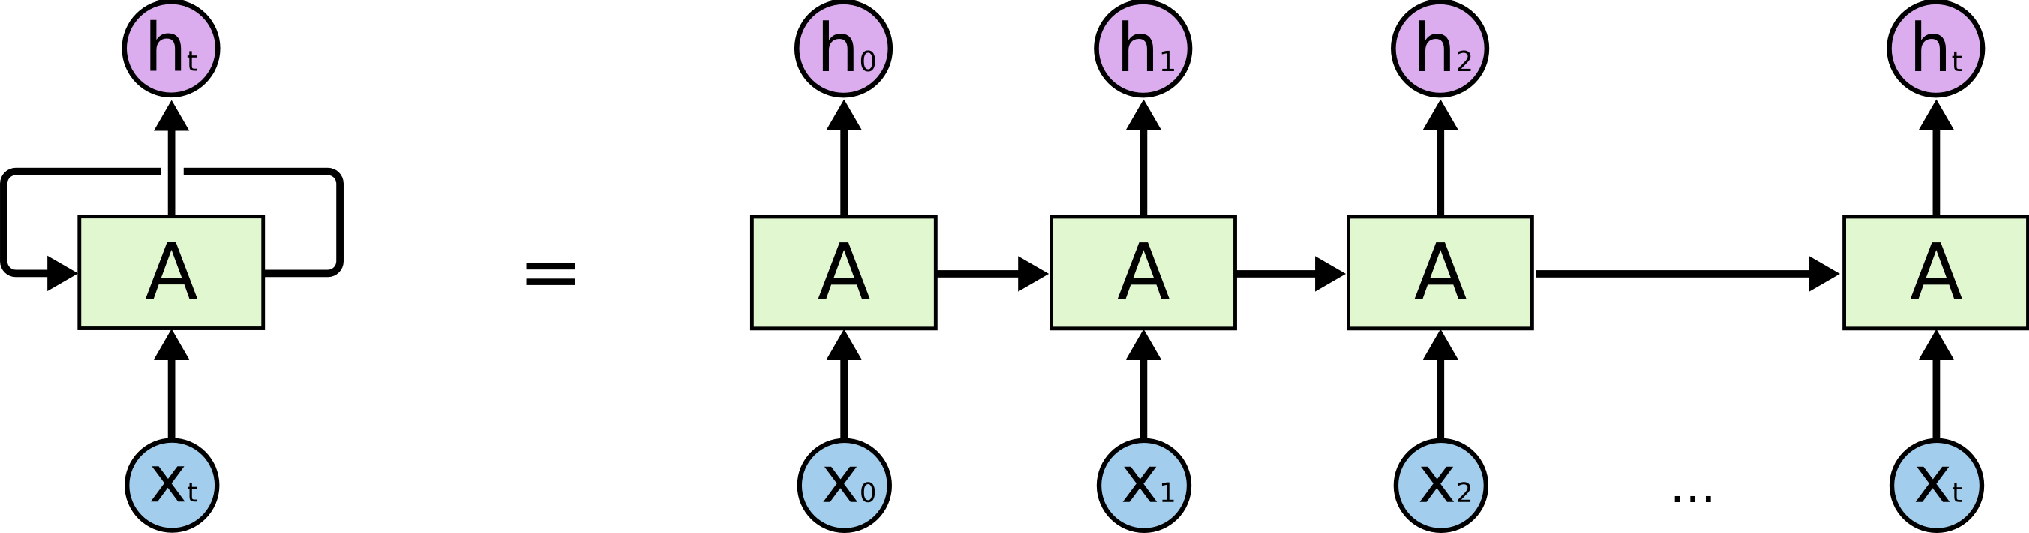
\includegraphics[width=\linewidth,keepaspectratio=true]{./figs/RNN-unrolled-pdf}
		\else
		\includegraphics[width=\linewidth,keepaspectratio=true]{./figs/RNN-unrolled-eps}
		\fi
		\caption{\small Schematic of a RNN \cite{olah}}
		\label{bck:rnn}
	\end{minipage}
\end{figure}

\section{BPTT and Vanishing Gradients}
The conventional method of training a feedforward neural network is a two step process. The first step called the \textbf{forward pass} when values fed at input layer pass through the hidden layers, are acted upon by (linear or non-linear) activations and come out at the output layer. In the second step called the \textbf{backward pass}  the error computed at the output layer (from the target output) flow backward through the network i.e. by applying the chain rule of differentiation, the error gradient at output layer, is computed with respect to all possible paths right upto input layer and then aggregated. This method of optimization in neural networks is called \textbf{backpropagation} \citep{Rumelhart1986}.

The optimization step i.e. the backward pass over the network weights is not just with regards to the parameters at the final time step but over all the time steps across which the weights (parameters) are shared. This is known as Back Propagation Through Time (BPTT) \citep{Werbos1990} and it gives rise to the problem of vanishing (or exploding) gradients in vanilla RNNs. This concept is better elaborated upon through equation in the following section.

\subsection{BPTT for Vanilla RNN}
\begin{equation}
\mathbf{\mathcal{L}\left(x,y\right)} = - \sum_{t}\left(y_t \log\hat{y_t}\right)
\end{equation}

%\begin{equation}
%\frac{\partial \mathbf{\mathcal{L}}}{\partial \alpha_t} = -\left(y_t-z_t\right)
%\end{equation}
The weight $W_{oh}$ is shared across all time steps. $\therefore$ adding the derivatives across the sequence:

\begin{equation}
\frac{\partial \mathbf{\mathcal{L}}}{\partial W_{oh}} = \sum_{t}\frac{\partial \mathbf{\mathcal{L}}}{\partial \hat{y_t}} \frac{\partial  \hat{y_t}}{\partial W_{oh}}
\end{equation}

%\begin{equation}
%\frac{\partial \mathbf{\mathcal{L}}}{\partial b_z} = \sum_{t}\frac{\partial \mathbf{\mathcal{L}}}{\partial z_t} %\frac{\partial  z_t}{\partial b_z}
%\end{equation}
For time-step t $\rightarrow$ t+1:

\begin{equation}
\frac{\partial \mathbf{\mathcal{L}}\left(t+1\right)}{\partial W_{hh}} = \frac{\partial \mathbf{\mathcal{L}}\left(t+1\right)}{\partial \hat{y}_{t+1}} \frac{\partial  \hat{y}_{t+1}}{\partial \mathbf{h}_{t+1}} \frac{\partial \mathbf{h}_{t+1}}{\partial W_{hh}}
\end{equation}

$W_{hh}$ is shared across time steps, we take the contribution from previous time steps as well, for calculating the gradient at time $t+1$. Summing over the sequence we get:

%\begin{equation}
%\frac{\partial \mathbf{\mathcal{L}}\left(t+1\right)}{\partial W_{hh}} = \frac{\partial %\mathbf{\mathcal{L}}\left(t+1\right)}{\partial \hat{y}_{t+1}} \frac{\partial  \hat{y}_{t+1}}{\partial \mathbf{h}_{t+1}} %\frac{\partial \mathbf{h}_{t+1}}{\partial \mathbf{h}_t} \frac{\partial \mathbf{h}_t}{\partial W_{hh}}
%\end{equation}

\begin{equation}
\frac{\partial \mathbf{\mathcal{L}}\left(t+1\right)}{\partial W_{hh}} = \sum_{\tau=1}^{t+1}\frac{\partial \mathbf{\mathcal{L}}\left(t+1\right)}{\partial \hat{y}_{t+1}} \frac{\partial  \hat{y}_{t+1}}{\partial \mathbf{h}_{t+1}} \frac{\partial \mathbf{h}_{t+1}}{\partial \mathbf{h}_{\tau}} \frac{\partial \mathbf{h}_{\tau}}{\partial W_{hh}}
\end{equation}

Summing over the whole sequence we get:

\begin{equation} \label{vanishing}
\frac{\partial \mathbf{\mathcal{L}}}{\partial W_{hh}} = \sum_{t}\sum_{\tau=1}^{t+1}\frac{\partial \mathbf{\mathcal{L}}\left(t+1\right)}{\partial \hat{y}_{t+1}} \frac{\partial  \hat{y}_{t+1}}{\partial \mathbf{h}_{t+1}} \frac{\partial \mathbf{h}_{t+1}}{\partial \mathbf{h}_{\tau}} \frac{\partial \mathbf{h}_{\tau}}{\partial W_{hh}}
\end{equation}

From equation \ref{vanishing} it is clear than the gradient of a RNN can be expressed as a recursive product of $\frac{\partial h_t}{\partial h_{t-1}}$. \textbf{If this derivative is $\ll 1$ or $\gg 1$, the gradient would vanish or explode respectively} when the network is trained over longer time-steps. In the former case error back-propagated would be too low to change the weights (the training would freeze) while in the latter it would never converge. 

Additionally revisiting equation \ref{nn-dynam} and rewriting it as follows:
\begin{equation}\label{ndq}	
h^{(t)} = f(x^{(t)}, h^{(t-1)}),
\end{equation}
it is not difficult to see that in the absence of an external input $x^{(t)}$ an RNN induces a a dynamical system. The RNN therefore can be viewed as a dynamical system with the input as an external force (map) that drives it. A dynamical system can posses a set of points which are invariant under any map. These points are called the \textbf{attractor states} of a dynamical system. These set of points can contain a single point (fixed attractor), a finite set of points (periodic attractor) or an infinite set of points (strange attractor). The type of attractor in a RNN unit depends on the initialization of the weight matrix for the hidden state \citep{Bengio1993}. Now under the application of map (input) if $\frac{\partial h_t}{\partial h_{k}}$ (for a large $t - k$ i.e. long term dependency), go to zero one can argue that the state $h_t$ is in the basin of one of the attractor states. This implies that in order to avoid the vanishing gradient problem a RNN cell must stay close to the \lq boundaries between basins of attraction \rq{} \citep{Pascanu2012}.

owing to this problem of vanishing (or exploding) gradients a vanilla RNN can't keep track of long term dependencies which is arguably critical for tasks such as speech synthesis, music composition or neural machine translation. The architectural modifications which solved the vanishing gradient problem and are the current de-facto RNN cell(s) are presented in the next section.


\iffalse
\begin{equation}
\frac{\partial \mathbf{\mathcal{L}}\left(t+1\right)}{\partial W_{hx}} = \frac{\partial \mathbf{\mathcal{L}}\left(t+1\right)}{\partial \mathbf{h}_{t+1}} \frac{\partial \mathbf{h}_{t+1}}{\partial W_{hx}}
\end{equation}

\begin{equation}
\begin{split}
\frac{\partial \mathbf{\mathcal{L}}\left(t+1\right)}{\partial W_{hx}} & = \frac{\partial \mathbf{\mathcal{L}}\left(t+1\right)}{\partial \mathbf{h}_{t+1}} \frac{\partial \mathbf{h}_{t+1}}{\partial W_{hx}} + \frac{\partial \mathbf{\mathcal{L}}\left(t+1\right)}{\partial \mathbf{h}_t} \frac{\partial \mathbf{h}_t}{\partial W_{hx}} \\
& = \frac{\partial \mathbf{\mathcal{L}}\left(t+1\right)}{\partial \mathbf{h}_{t+1}} \frac{\partial \mathbf{h}_{t+1}}{\partial W_{hx}} + \frac{\partial \mathbf{\mathcal{L}}\left(t+1\right)}{\partial \mathbf{h}_{t+1}} \frac{\partial \mathbf{h}_{t+1}}{\partial \mathbf{h}_t}\frac{\partial \mathbf{h}_t}{\partial W_{hx}}
\end{split}\end{equation}

\begin{equation}
\frac{\partial \mathbf{\mathcal{L}}\left(t+1\right)}{\partial W_{hx}} = \sum_{\tau=1}^{t+1} \frac{\partial \mathbf{\mathcal{L}}\left(t+1\right)}{\partial \mathbf{h}_{t+1}} \frac{\partial \mathbf{h}_{t+1}}{\partial \mathbf{h}_{\tau}} \frac{\partial \mathbf{h}_{\tau}}{\partial W_{hx}}
\end{equation}

\begin{equation}
\frac{\partial \mathbf{\mathcal{L}}}{\partial W_{hx}} = \sum_{t} \sum_{\tau=1}^{t+1} \frac{\partial \mathbf{\mathcal{L}}\left(t+1\right)}{\partial \hat{y}_{t+1}} \frac{\partial \hat{y}_{t+1}}{\partial \mathbf{h}_{t+1}} \frac{\partial \mathbf{h}_{t+1}}{\partial \mathbf{h}_{\tau}} \frac{\partial \mathbf{h}_{\tau}}{\partial W_{hx}}
\end{equation}
\fi

\section{Gated RNNs}
The problem of vanishing (or exploding) gradients makes a vanilla RNN unsuitable for long term dependency modeling. However if for instance the RNN was to compute an identity function then the gradient computation wouldn't vanish or explode since the Jacobian is simply an identity matrix. Now while an identity initialization of recurrent weights by itself isn't very interesting it brings us to the underlying principle behind gated architectures i.e. the mapping from memory state at one time step to the next is close to identity function.

\begin{figure}[ht] 
	\begin{subfigure}[b]{0.5\linewidth}
		\centering
		\ifpdf
		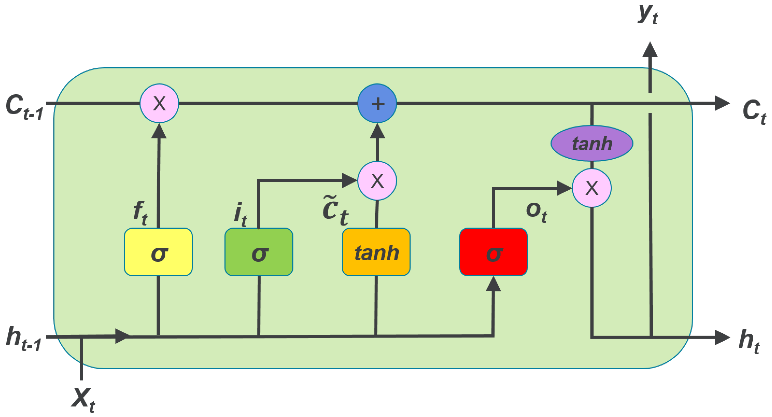
\includegraphics[width=0.95\linewidth]{./figs/Lstm-pdf}
		\else
		\includegraphics[width=0.95\linewidth]{./figs/Lstm-eps}
		\fi
		\caption{LSTM\citep{Zheng2017}}
		\label{lstm} 
		\vspace{4ex}
	\end{subfigure}%% 
	\begin{subfigure}[b]{0.5\linewidth}
		\centering
		\ifpdf
		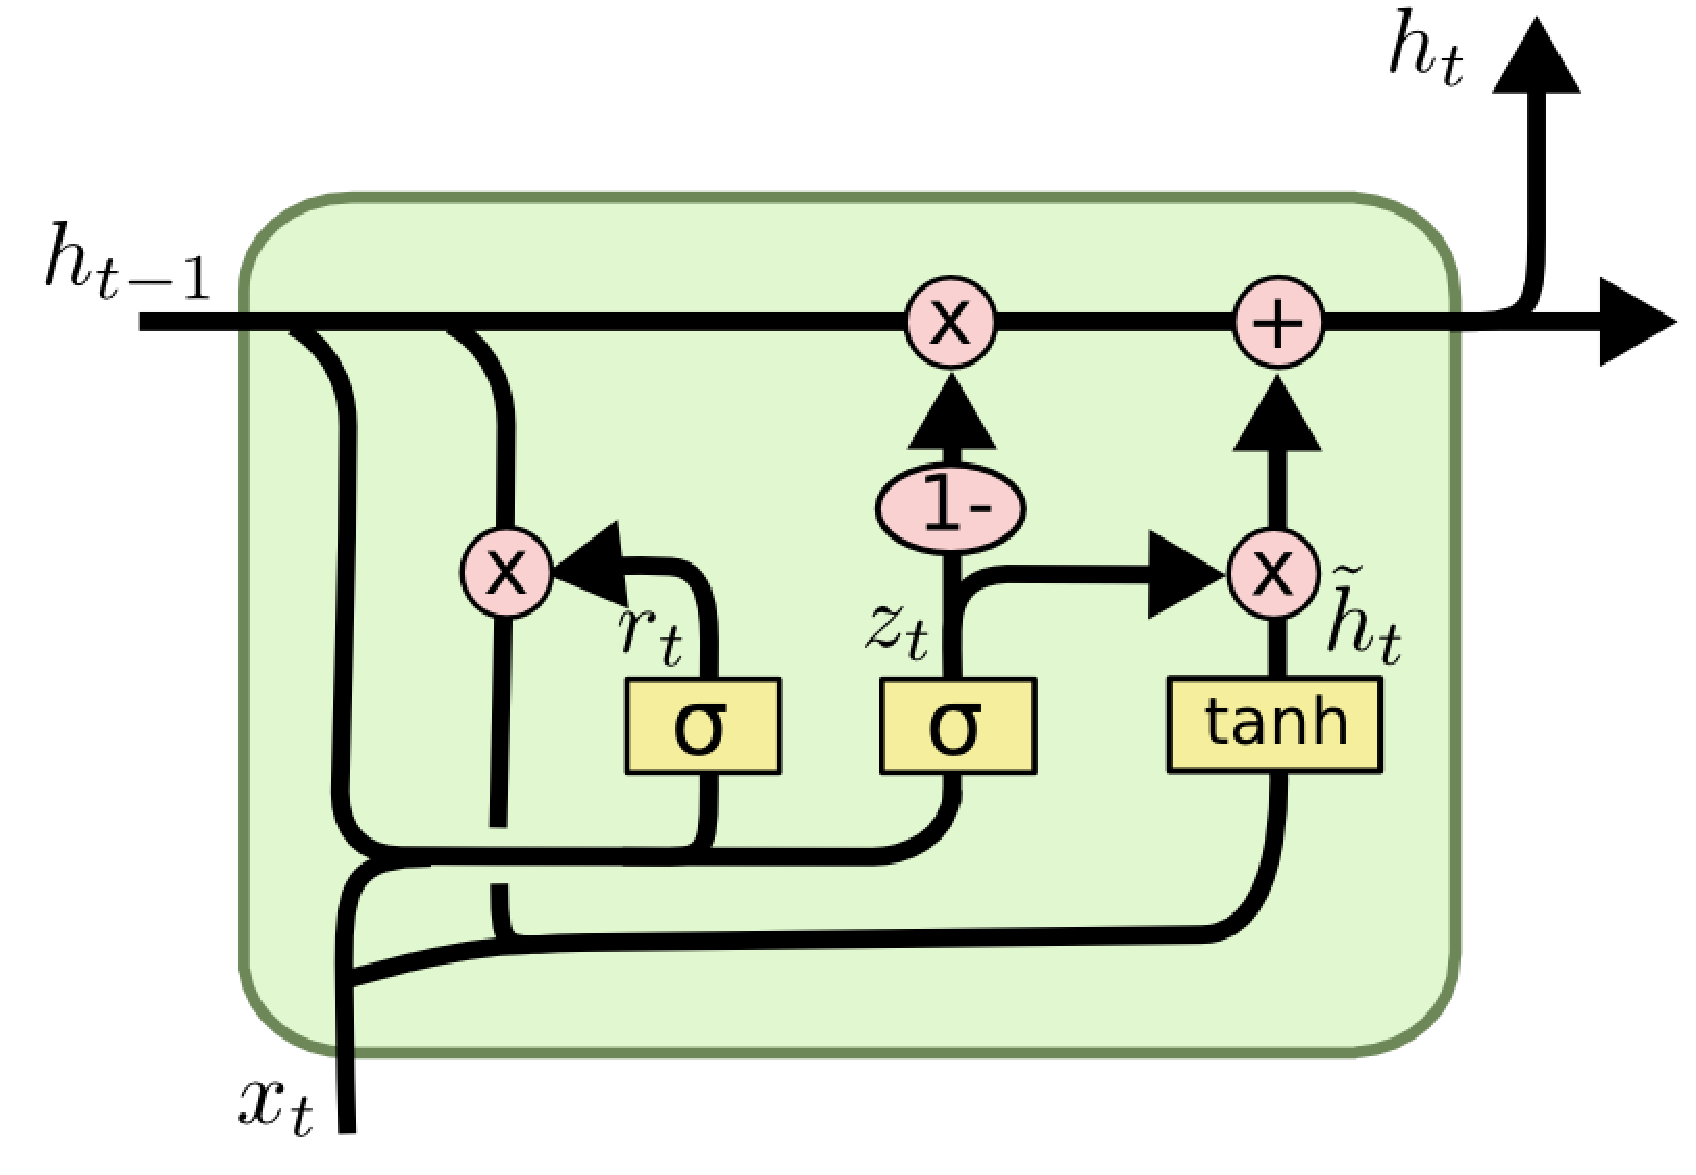
\includegraphics[width=0.95\linewidth]{./figs/Gru-pdf}
		\else
		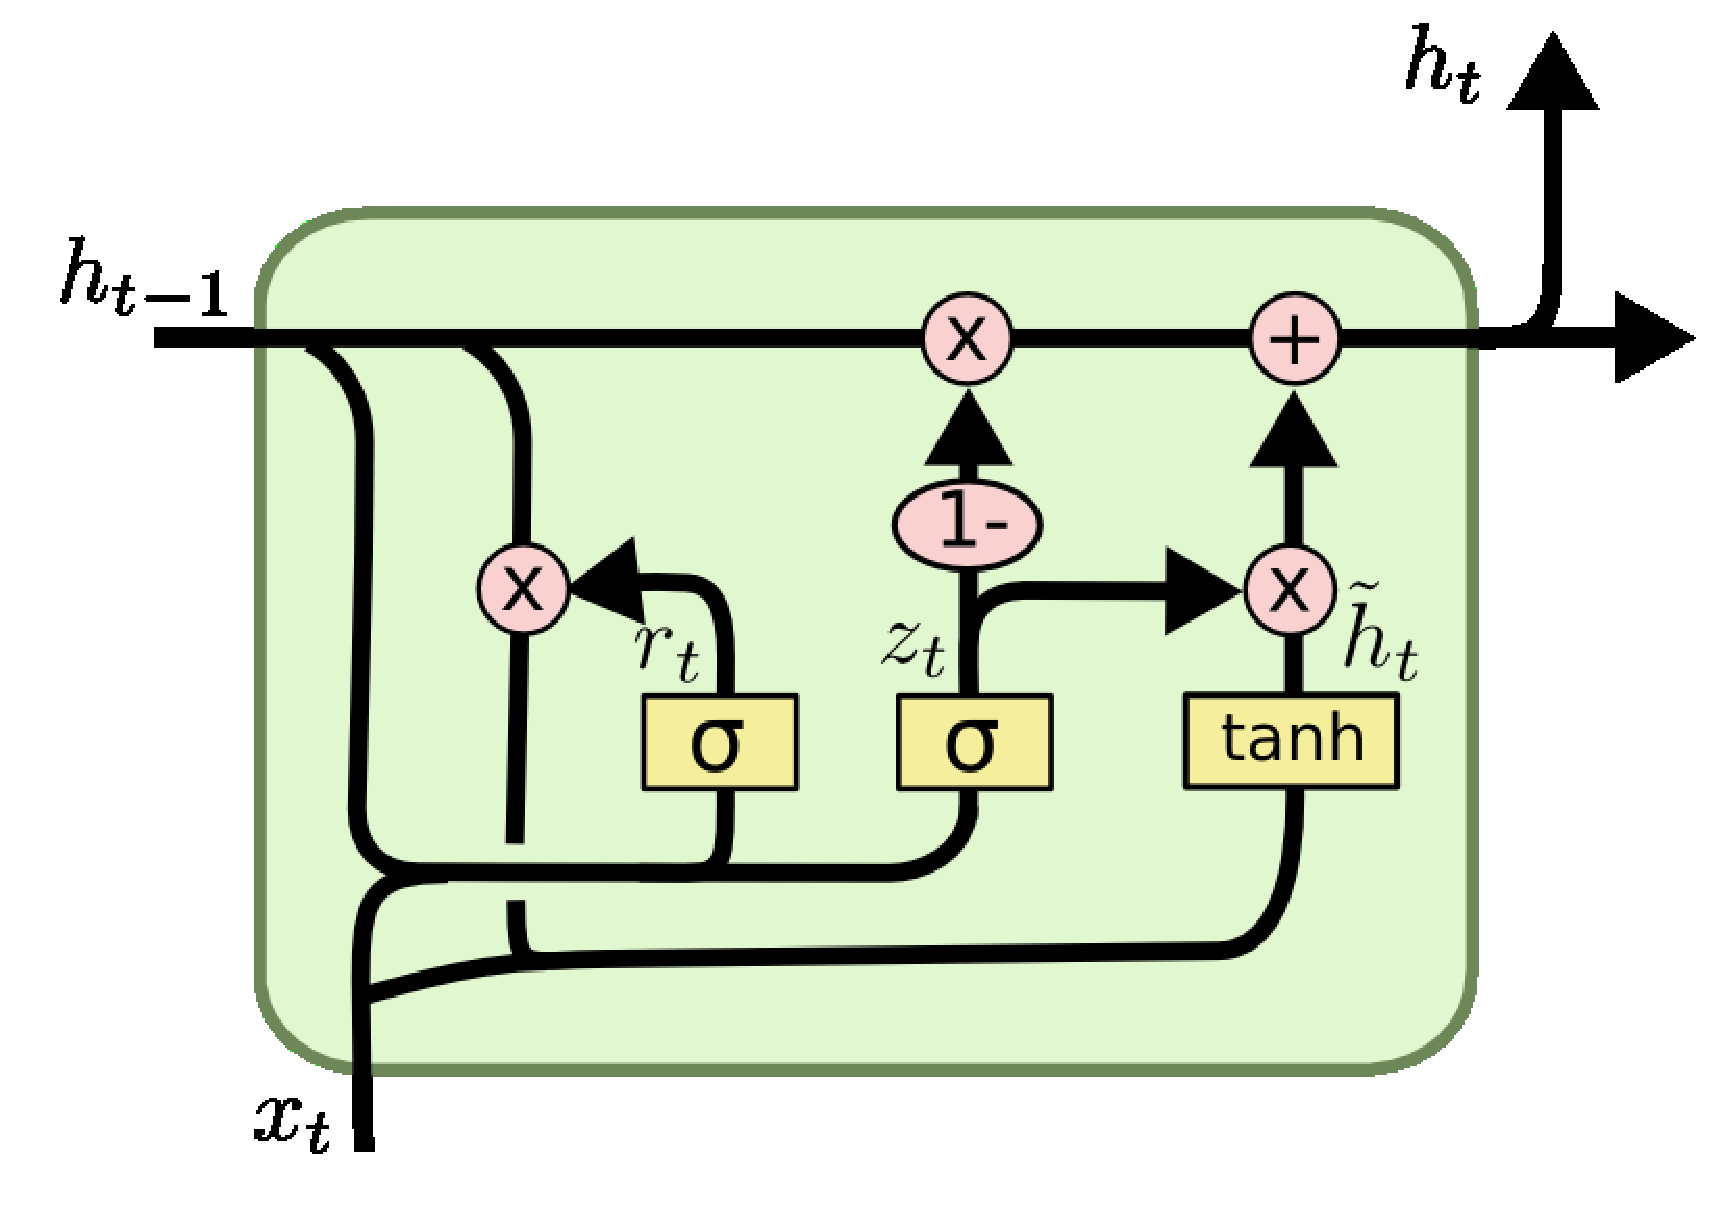
\includegraphics[width=0.95\linewidth]{./figs/Gru-eps}
		\fi 
		\caption{GRU \citep{olah}} 
		\label{gru}  
		\vspace{4ex}
	\end{subfigure}
	\caption{Gated RNNs}
	\label{conf}
\end{figure}

\subsection{LSTM}
Long Short Term Memory (LSTM) introduced by \cite{LSTM} is one of the two most widely used gated RNN architectures in use today. The fact that it has survived all the path-breaking innovations in the field of deep learning for over twenty years to still be the state of the art in sequence modeling speaks volumes about the architecture's ingenuity and strong fundamentals. 

The fundamental principle behind the working of a LSTM is, alter the memory vector only selectively between time steps such that the memory state is preserved over long distances. The architecture is explained as follows:


\begin{equation}
i= \sigma(x_t U^{(i)}, m_{t-1}W^{(i)})
\end{equation}

\begin{equation}
f= \sigma(x_t U^{(f)}, m_{t-1}W^{(f)})
\end{equation}

\begin{equation}
o= \sigma(x_t U^{(o)}, m_{t-1}W^{(o)})
\end{equation}

\begin{equation}
\widetilde {c_t}= \tanh(x_t U^{(g)}, m_{t-1}W^{(g)})
\end{equation}

\begin{equation}
c_t = c_{t-1} \odot f + \widetilde{c_t} \odot i
\end{equation}

\begin{equation}
m_t = tanh(c_t) \odot o
\end{equation}

\begin{itemize}
	\item \textbf{input gate $i^{(t)}$:} The input computes a new cell state based on the current input and the previous hidden state and decides how much of this information to "let through" via. a sigmoid activation.
	\item \textbf{forget gate $f^{(t)}$:} The forget gate decides what to remember and what to forget for the new memory based on the current input and the previous hidden state.The sigmoid activation acts like a switch where 1 implies remember everything while 0 implies forget everything.
	\item \textbf{output gate $o^{(t)}$:} The output gate then determines determines (via a sigmoid activation) the amount of this internal memory to be exposed to the top layers (and subsequent timesteps) of the network.
	\item \textbf{The input modulation $g^{(t)}$} computed based on the present input and the previous hidden state (which is exposed to the output) yields candidate memory for the cell state via a tanh layer. The hadamard products of input gate and candidate memories is added to the hadamard product of forget gate and previous cell state to yield the new cell state.
	\item \textbf{hidden state $m^{(t)}$:} A hadamard product of the hyperbolic tangent of current cell state and output gate yields the current hidden state.
\end{itemize}

\subsection{GRU}
The Gated Recurrent Unit (GRU) introduced by \cite{GRU} are a new type of gated RNN architecture whose details are as follows:

\begin{equation}
z_t= \sigma(x_t U^{(z)}, m_{t-1}W^{(z)})
\end{equation}

\begin{equation}
r_t= \sigma(x_t U^{(r)}, m_{t-1}W^{(r)})
\end{equation}

\begin{equation}
\widetilde {m_t}= \tanh(x_t U^{(g)},r_t \odot m_{t-1}W^{(g)})
\end{equation}

\begin{equation}
m_t= (1-z_t)m_{t-1} + z_t\widetilde{m_t} %\sigma(x_t U^{(i)} m_{t-1}W^{(i)})
\end{equation}

\begin{itemize}
	\item \textbf{update gate $z_{(t)}$:} The update gate is the filter which decides how much of the activations/memory to be update at any given time step.
	\item \textbf{reset gate $r_{(t)}$:} The reset gate is similar to the forget gate in a LSTM. When its value is close to zero it allows the cell to forget the previously computed state.
	\item \textbf{The input modulation $g_{(t)}$} just as in the case of the LSTM  serves the purpose of yielding candidate memories for the new cell state.
	\item \textbf{hidden state $m_{(t)}$:} The current hidden state is a weighted average of the previous hidden state and the candidate hidden state weighted by (1 - update gate) and the (update gate) respectively.
\end{itemize}


While there are a lot of similarities between a GRU and a LSTM the most striking difference is the lack of an output gate in a GRU. Unlike a LSTM a GRU doesn't control how much of its internal memory to expose to the rest of the units in the network. The GRU therefore has fewer parameters due to the lack of an output gate and is computationally less intensive in comparison to a LSTM.

\section{Seq2Seq Models}\label{background:s2s}
\begin{figure}
	\begin{minipage}[t]{\textwidth}
		\ifpdf
		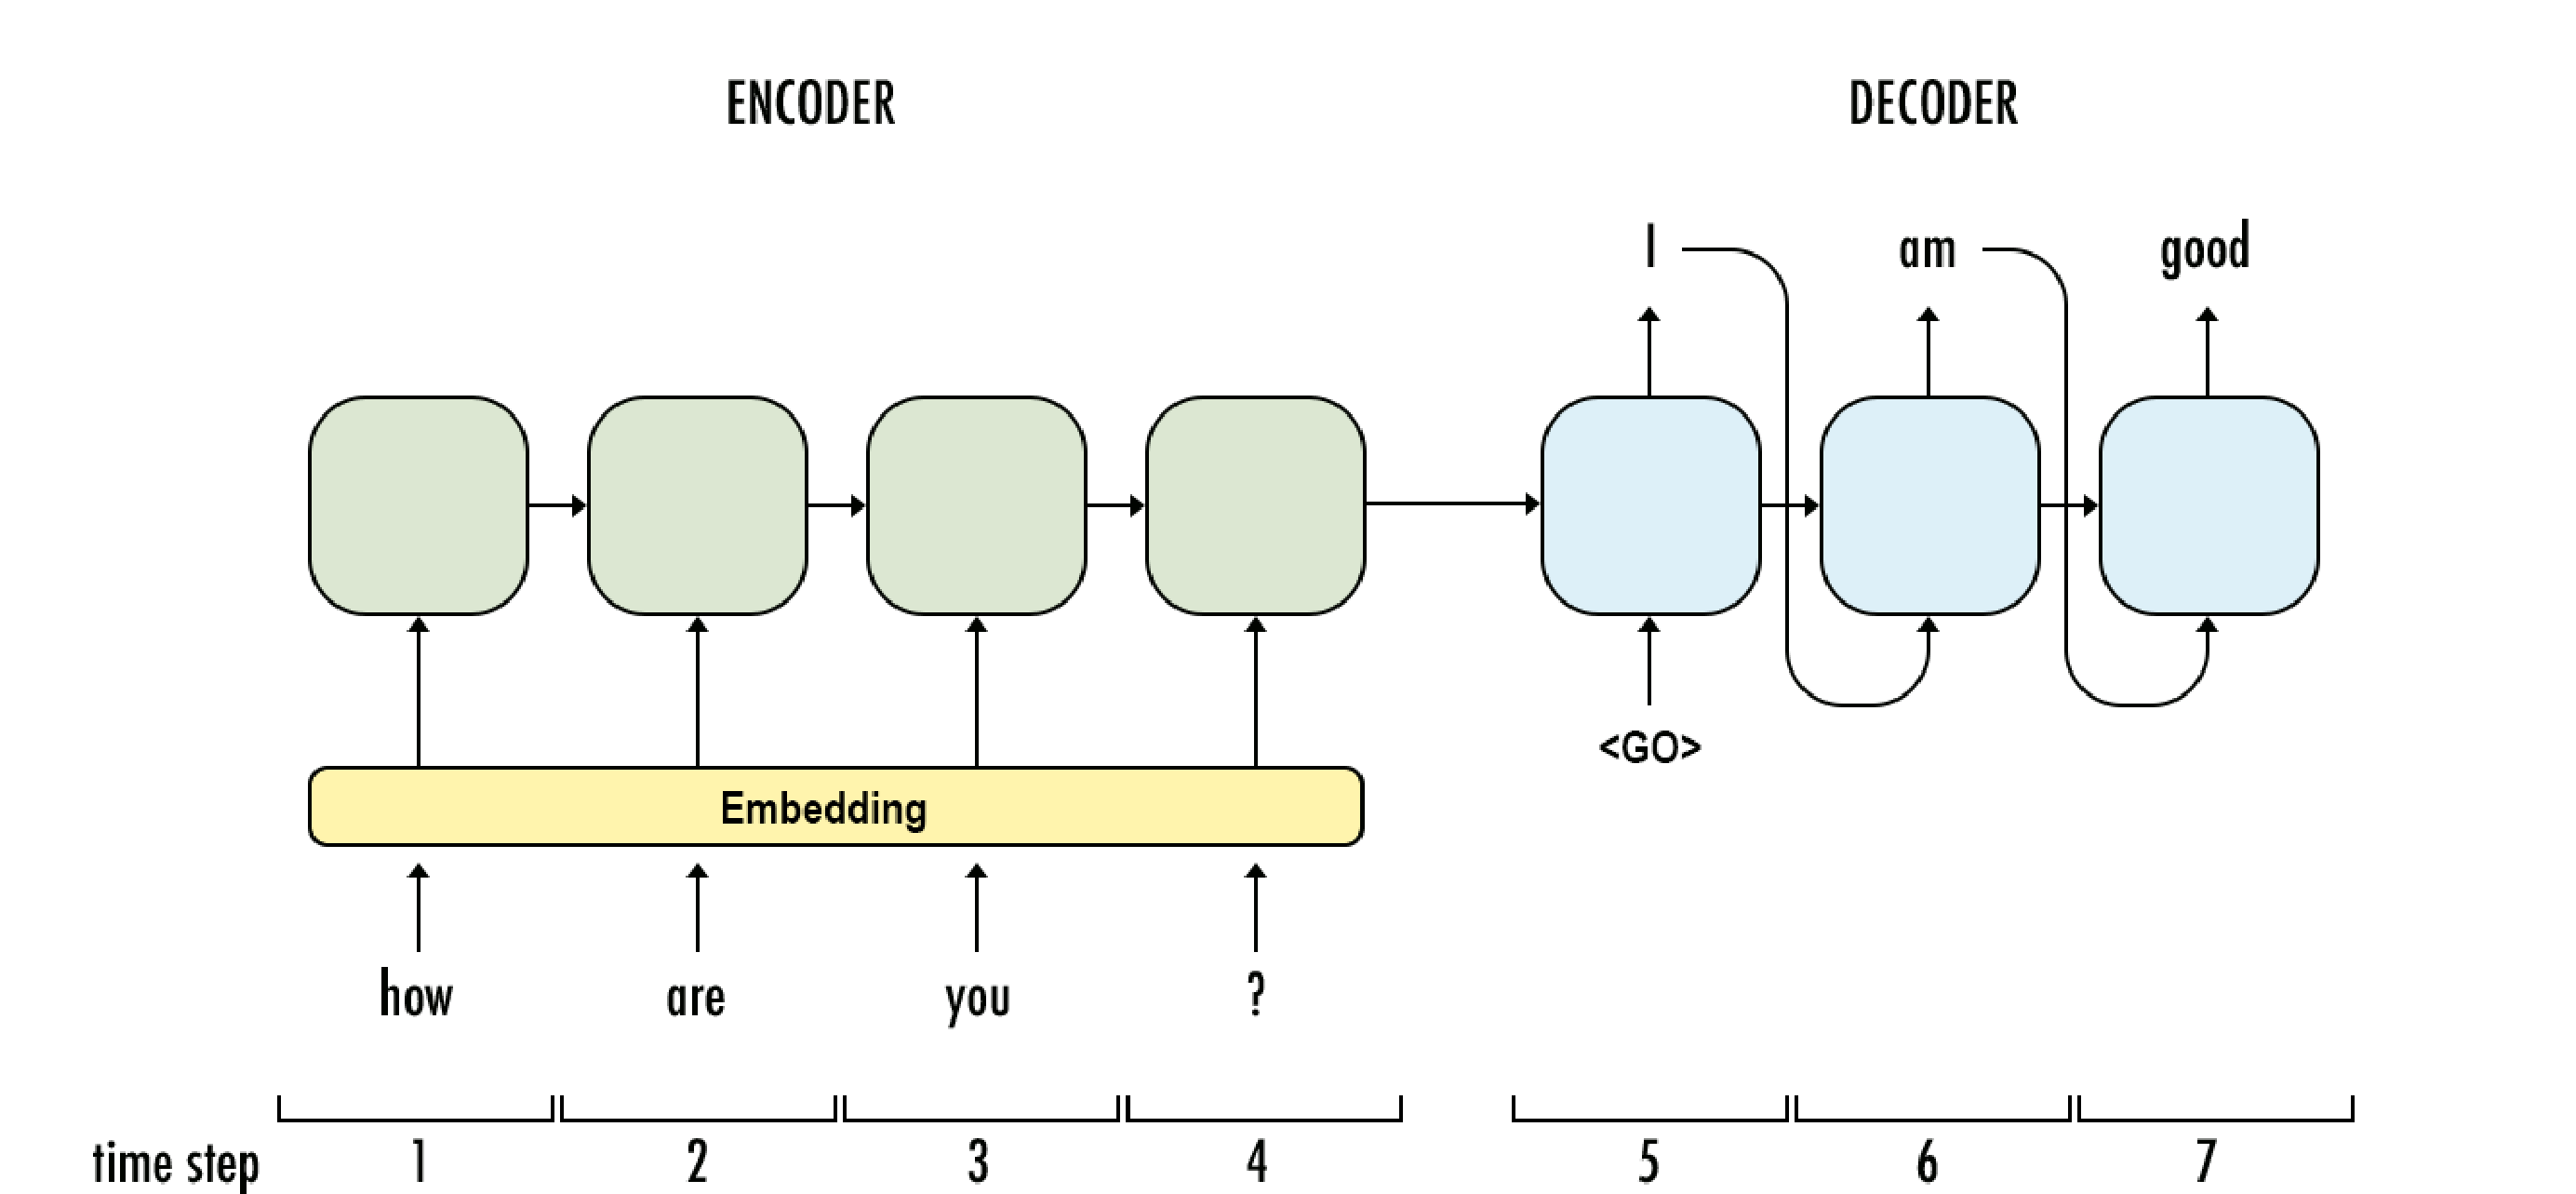
\includegraphics[width=\linewidth,keepaspectratio=true]{./figs/s2s-pdf}
		\else
		\includegraphics[width=\linewidth,keepaspectratio=true]{./figs/s2s-eps}
		\fi
		\caption{Schematic of a Seq2Seq \citep{manish}}
		\label{bck:s2s}
	\end{minipage}
\end{figure}

Sequence-to-sequence (seq2seq) models introduced by \cite{Sutskever2014}, \cite{GRU} are a class of probabilistic generative models that let us learn the mapping from a variable length input to a variable length output. While initially conceived for machine translation, they have been applied successfully to the tasks of speech recognition, question answering and text summarization \citep{Vinyals2015} \citep{anderson2018bottom} \citep{lu2017knowing}.

Neural networks have been shown to be excellent at learning rich representation from data without the need for extensive feature engineering \citep{Hinton2006}. RNNs are especially adept at learning features and long term dependencies in sequential data (section \ref{RNN}). The simple yet effective idea behind a seq2seq model is learning a fixed size (latent) representation of a variable length input and then generating a variable length output by conditioning it on this latent representation and the previous portion of the output sequence.

\begin{equation} \label{decoder:eqn1}
	h^{(t)} = f(x^{(t)}, h^{(t-1)}, v)
\end{equation}

\begin{equation} \label{decoder:eqn2}
	P(x^{(t+1)}|x^{(t)}, x^{(t-1)},.....,x^{(1)}) = g(x^{(t)}, h^{(t)}, v)
\end{equation}

It can be seen from equation \ref{decoder:eqn2} that the decoder is auto-regressive with the long term temporal dependencies captured in its hidden state. The term $\mathbf{v}$ represents the summary of the entire input state compressed into a fixed length vector (last hidden state of encoder) viz. the \textbf{latent space}. This encoder- decoder network is then jointly trained via. cross entropy loss between the target and the predicted sequence.

\subsection{Se2Seq with Attention}\label{mtv:attn}
It was shown by \cite{Cho2014} that the performance of a basic encoder-decoder models as explained in \ref{background:s2s} is inversely related to the increase in length of the input sentence. Therefore in lines with concepts of the selective attention and attentional blink in human beings, \cite{Bahdanau2014} and later  \cite{Luong2015} showed that soft selection from source states where most relevant information can be assumed to be concentrated during a particular translation step in NMT leads to improved performance. In the Bahdanau \citep{Bahdanau2014} framework of attention, the equations \ref{decoder:eqn1} and \ref{decoder:eqn2} are modified as follows:

\begin{equation}\label{attn:eqn1}
h^{(t)} = f(x^{(t)}, h^{(t-1)}, c^{(t)}),
\end{equation}

\begin{equation} \label{attn:eqn2}
P(x^{(t+1)}|x^{(t)}, x^{(t-1)},.....,x^{(1)}) = g(x^{(t)}, h^{(t)}, c^{(t)}).
\end{equation}

Here unlike the traditional seq2seq model the probability of emission of the output at time step $t$ isn't conditioned on a fixed summary representation $\mathbf{v}$ of the input sequence. Rather it is conditioned on a context vector $\mathbf{c^{(t)}}$ which is distinct at each decoding step. The context vector is calculated using a sequence of encoder outputs $(s^1, s^2, ....,s^N)$ to which the the input sequence is mapped such that an encoder output $s^i$ contains a representation of the entire sequence with maximum information pertaining to the $i_{th}$ word in the input sequence. The context vector is then calculated as follows:

\begin{equation}\label{attn:eqn3}
c^{(t)}  = \sum_{j=1}^N \alpha_{tj} s^j,
\end{equation}
where:
\begin{equation}\label{attn:eqn4}
\alpha_{tj} = \text{softmax}(e(h^{(t-1)}, s^j)).
\end{equation}
where $e$ is a alignment/matching/similarity measure between the decoder hidden state $h^{(t-1)}$ i.e. just before the emission of output $x^{(t)}$. The alignment function can be a dot product of the two vectors or a feed-forward network that is jointly trained with the encoder-decoder model. The $\alpha_{tj}$ is an attention vector that weighs the encoder outputs at a given decoding step. \cite{Vaswani2017} view the entire process of attention and context generation as a series of functions applied to the tupe (query, key, value), with the first step being an \textbf{attentive read} step where a scalar matching score between the query and key ($h^{(t-1)}, s^j$) is calculated followed by computation of attention weights $\alpha_{tj}$. Weighted averaged of the \lq values{}\rq\ using the attention weights is then done in the \textbf{aggregation} step.  


\section{Pondering}

\begin{figure}
	\begin{minipage}[t]{\textwidth}
		\ifpdf
		\includegraphics[width=\linewidth,keepaspectratio=true]{./figs/act-pdf}
		\else
		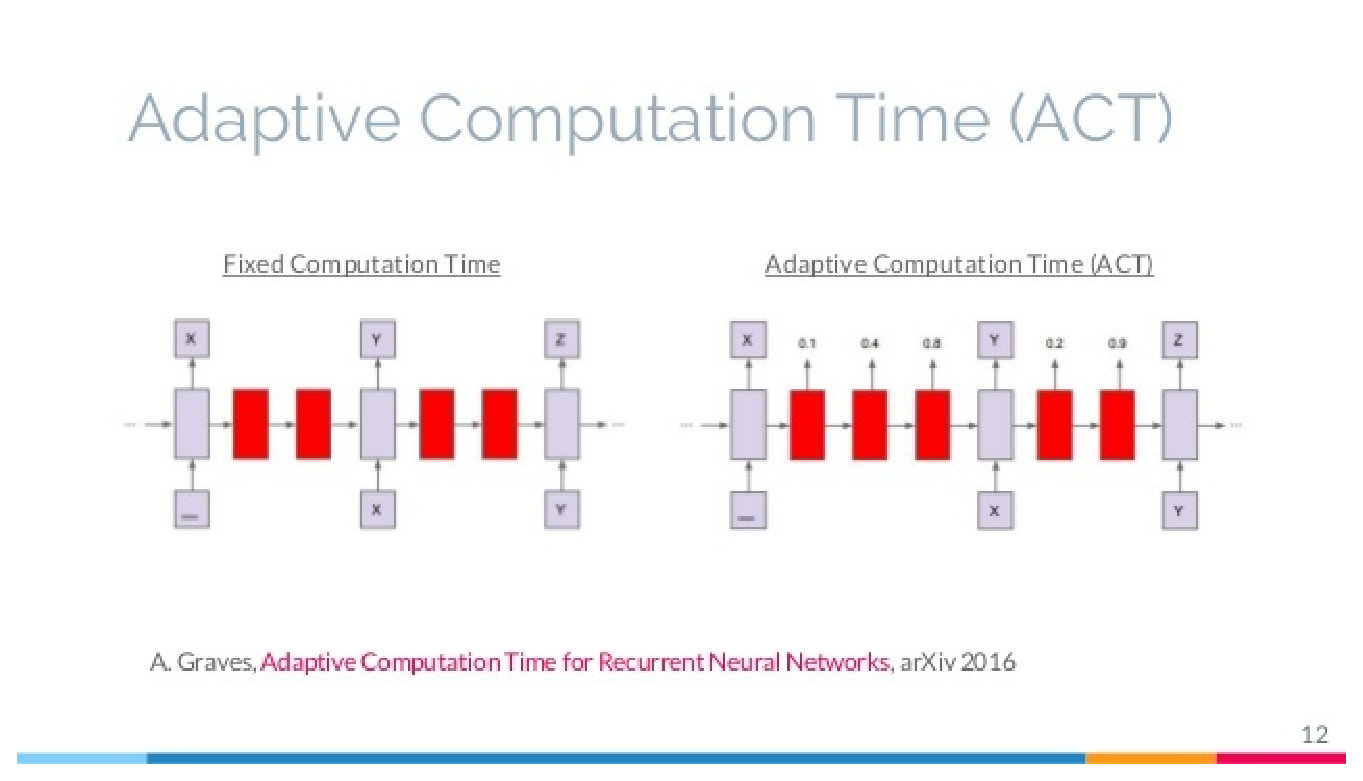
\includegraphics[width=\linewidth,keepaspectratio=true]{./figs/act-eps}
		\fi
		\caption{\small Adaptive Computation Time}
		\label{mtv:ponder}
	\end{minipage}
\end{figure}

The task of positioning a problem and solving belong to different classes of time complexity with the latter requiring more time than the former. \cite{Graves2016} argued that for a given RNN unit it is reasonable to allow for variable computation time for each input in a sequence since some parts of the input might be inherently more complex than the others and thereby require more computational steps. A very good example of this would be \textit{spaces between words and ends of sequences}. 

Human beings overcome similar obstacles by allocating more time to a difficult problem as compared to a simpler problem. Therefore a naive solution would be to allow a RNN unit to have a large number of hidden state transitions (without penalty of amount of computations performed) before emitting an output on a given input. The network would therefore learn to allocate as much time as possible to minimize its error thereby making it extremely inefficient. \cite{Graves2016} proposed the concept of \textbf{adaptive computation time} to have a trade-off between accuracy and computational efficacy in order to determine the minimum number of state transitions required to solve a problem \footnote{Theoretically this is akin to halting on a given problem or finding the Kolmogorov Complexity of the data, both of which are unsolvable}.

\textbf{A}daptive \textbf{C}omputation \textbf{T}ime (ACT) achieves the above outlined goals by making two simple modifications to a conventional RNN cell, which are presented as follows:

\subparagraph{Sigmoidal Halting Unit} If we revisit the equations of a vanilla RNN from section \ref{ndq}, they can be summarized as:
\begin{equation}
\begin{aligned}
h_t &= f(Ux_t + Wc_{t-1}), \\
y_t &= g(Vc_t).
\end{aligned}
\end{equation}
ACT now allows for \textit{variable state transitions} ($c_t^1, c_t^2,...., c_t^{N(t)}$) and by extension an \textit{intermediate output sequence} ($y_t^1, y_t^2,...., y_t^{N(t)}$) at any given input step \textit{t} as follows:
\begin{equation}
\begin{aligned}
c_t^n &= \begin{cases} f(Ux_t^1 + Wc_{t-1})\ \text{if}\ n = 1 \\ f(Ux_t^n + Wc_t^{n-1})\ \text{if}\ n \neq 1  \end{cases}, \\
y_t^n &= g(Vc_t^n).
\end{aligned}
\end{equation}

A sigmoidal halting unit (with its associated weight matrix $S$) is now added to the network in order to yield a halting probability $p_t^n$ at each state transition as follows:
\begin{equation}
\begin{aligned}
h_t^n &= \sigma(Sc_t^n), \\
p_t^n &= \begin{cases} R(t)\ \text{if}\ n = N(t) \\ h_t^n\ \text{if}\ n \neq N(t)  \end{cases},
\end{aligned}
\end{equation}
where:
\begin{equation}
\begin{aligned}
N(t) &= min\{m : \sum_{n=1}^m h_t^n \geq 1 - \epsilon\}, \\
R(t) &= 1 - \sum_{n=1}^{N(t)-1} h_t^n,
\end{aligned}	
\end{equation}
and $\epsilon$ is a small constant.

Each ($n^{th}$) hidden state and output transition at input state \textit{t} are now weighted by the corresponding halting probability $p_t^n$ and summed over all the updates $N(t)$ to yield the final hidden state $c_t$ and output $y_t$ at a given input step. Figure \ref{mtv:ponder} outlines the difference between a standard RNN cell and an ACT RNN cell by showing variable state transitions for input $x$ and $y$ respectively with the corresponding probability associated with each update step. It can be noted that $\sum_n=1^N(t) p_t^n = 1\ \text{and}\ 0 \leq p_t^n \leq 1\ \forall n$, and therefore it constitutes a valid probability distribution.

\subparagraph{Ponder Cost} If we don't put any penalty on the number of state transitions then the network would become computationally inefficient and would \lq \textbf{ponder}{}\rq\ for long times even on simple inputs in order to minimize its error. Therefore in order to limit the variable state transitions ACT adds a ponder cost $\mathcal{P}(x)$ to the total loss of the network as follows:
given an input of length $T$ the ponder cost at each time step $t$ is defined as:

\begin{equation}
\rho_t = N(t)/ +\ R(t)
\end{equation}

\begin{equation}
\begin{aligned}
\mathcal{P}(x) &= \sum_{t=1}^T \rho_t, \\
\widetilde{\mathcal{L}}(x,y) &= \mathcal{L}(x,y) + \tau\mathcal{P}(x),
\end{aligned}	
\end{equation}
where $\tau$ is a penalty term hyperparameter (that needs to be tuned) for the ponder loss.

\section{Formal Language Theory}\label{flt}
The field of formal language theory (FLT) concerns itself with the syntactic structure of a formal language (=set of strings) without much emphasis on the semantics. More precisely a formal language $L$ is a sequence of strings with the constituent units/words/morphemes taken from a finite vocabulary $\Sigma$. It is more apt to define the concept of a formal grammar before proceeding further. A formal grammar $G$ is a quadruple $\langle \Sigma, NT, S, R \rangle$ where $\Sigma$ is a finite vocabulary as previously defined, $NT$ is a finite set of non-terminals, $S$ the start symbol and $R$ the finite set of valid production rules. A production rule can be expressed as $\alpha \rightarrow \beta$ and can be understood as a substitution of $\alpha$ with $\beta$ with $\alpha, \beta$ coming from the following sets for a \textbf{valid} production rule:

\begin{equation}\label{term-nonterm}
	\alpha \in (\Sigma \cup NT)^{*}NT(\Sigma \cup NT)^{*} \qquad \beta \in (\Sigma \cup NT)^{*} \footnote{The \lq *\rq\ denotes Kleene Closure and for a set of symbols say $X$, $X^{*}$ denotes a set of all strings that can be generated using symbols from X, including the empty string $\epsilon$ }.
\end{equation}

From equation \ref{term-nonterm} it is easy to see that the left hand side of the production rule can never be null ($\epsilon$) and must contain at-least one non-terminal. Now a formal language $L(G)$ can be defined as the set of all strings  \textit{generated} by grammar $G$ such that the string consists of morphemes only from $\Sigma$, and has been generated by a finite set of rule ($R$) application after starting from $S$. The \textit{decidability} of a grammar, is the verification -by a Turing machine or another similar computational construct e.g. a finite state automaton (FSA)- of whether a given string has been generated by that grammar or not (the \textit{membership} problem). A grammar is decidable if the membership problem can be solved for all given strings.

\begin{figure}
	\begin{minipage}[t]{\textwidth}
		\ifpdf
		\includegraphics[width=\linewidth,keepaspectratio=true]{./figs/chomsky_h-pdf}
		\else
		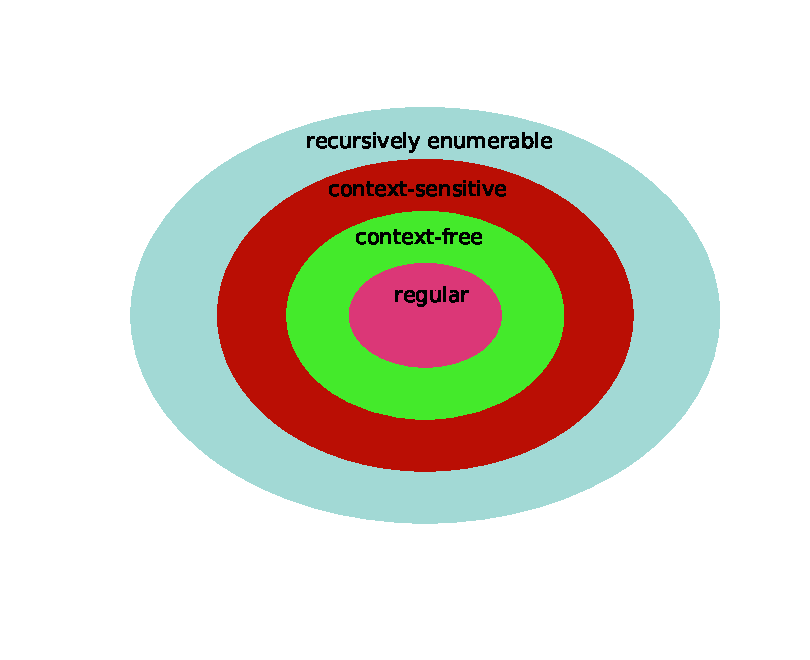
\includegraphics[width=\linewidth,keepaspectratio=true]{./figs/chomsky_h-eps}
		\fi
		\caption{\small Chomsky Hierarchy}
		\label{mtv:ch}
	\end{minipage}
\end{figure}

\subsection{Chomsky Hierarchy}\label{flt:ch}
\cite{Chomsky1956} introduced a nested hierarchy for different formal grammars of the form $C_1 \subsetneq C_2 \subsetneq C_3 \subsetneq C_4$ as shown in figure \ref{mtv:ch}. The different classes of grammar are progressively strict subsets of the class just above them in the hierarchy. These classes are not just distinguished by their rules or the languages they generate but also on the computational construct needed to decide the language generated by this grammar. We now take a closer look at the classes in this hierarchy. Please note that for each of these classes the grammar definition is G = $\langle \Sigma, NT, S, R \rangle$.
\subparagraph{Recursively Enumerable.} Any grammar characterized by no constraints on the production rules $\alpha \rightarrow \beta$. Therefore any valid grammar is recursively enumerable. The language generated by this grammar is called recursively enumerable language (REL) and is accepted by a Turning Machine.
\subparagraph{Context-Sensitive.} In this grammar the left hand side of the production rule i.e. $\alpha$ has the same definition as above (equation \ref{term-nonterm}) but an additional constraint of the form $|\alpha| \leq |\beta|$ is now imposed on the grammar. This is turn leads to $\beta \in (\Sigma \cup NT)^{+}$, i.e. the right hand side of the production rule is now under Kleene Plus closure \footnote{$(\Sigma \cup NT)^{+} = (\Sigma \cup NT)^{*} - \epsilon$}. The non production of $\epsilon$ in context-sensitive grammars poses a problem to the hierarchy because the production of null symbol isn't restricted in its subclasses. While keeping the hierarchy as it is \cite{Chomsky1963} resolved this paradox by defining noncontracting grammmar which is \textit{weakly equivalent}(generates same set of string) to the context sensitive grammar. Noncontracting grammars allow the $S \rightarrow \epsilon$ production. Context sensitive grammars generate context sensitive languages which are accepted by a linear bounded turing machine. While in principle this grammar is decidable, the problem is PSPACE hard and can be so complex, that it is practically intractable \citep{Jager2012}. 
\subparagraph{Context-Free.} Such a grammar is described by production rules of the form $A \rightarrow \alpha$ where $A \in NT$ and $\alpha \in (\Sigma \cup NT)^{*}$, such that $|A|=1$.  Context free grammar lead to context free languages (CFL) which are hierarchical in structure, albeit it is possible that same CFL can be described by different context free grammars, leading to different hierarchical syntactic structures of the language. A CFG is decidable in cubic time of length of string by push down FSA. A psuh down automaton employs a running stack of symbols to decide its next transition. The stack can also be manipulated as a side effect of the state transition.
\subparagraph{Regular.} Characterized by production rules of the form $A \rightarrow \alpha or A \rightarrow \alpha B$ where $\alpha \in \Sigma^{*}$ and $(A, B) \in NT$. . The non terminal in production can therefore be viewed as the next state(s) of a finite state automaton (FSA) while the terminals are the emissions. Regular grammars are decidable in linear time of length of string by a FSA.


\subsection{Subregular Hierarchy}\label{flt:sh}
The simplest class of languages encountered in section \ref{flt:ch} were regular languages that can be described using a FSA. \cite{Jager2012} however argue that the precursor to human language faculty would require lower cognitive capabilities and it stands to reason that even simpler structures can exist in the \lq Regular\rq{} domain. They therefore introduced the concept of subregular languages. If a language can be described by a mechanism even simpler than the FSA then it is a subregular language introduced by While far from the expressive capabilities of regular languages which in turn are the least expressive class in the Chomsky hierarchy, subregular languages provide an excellent benchmark to test basic concept learning and pattern recognition ability of any intelligent system.

\subparagraph{Strictly local languages.} We start with a string $w$ and we are given a lookup table of k-adjacent characters known as \textit{k-factors}, drawn from a particular language. The lookup table therefore serves the role of the language description. A language is \textit{k}-local, if every \textit{k}-factor seen by a \textit{scanner} with a windows of size $k$ sliding over the string $w$, is included in the aforementioned lookup-table. A $SL_k$ language description, is just the set of k-factors prefixed and suffixed by a start and end symbol, say $\#$. E.g. $SL_2 = \{\#A,AB,BA,B\#\}$   

\subparagraph{Locally k-testable languages.} Instead of sliding a scanner over \textit{k}-factors we consider all the \textit{k}-factors to be atomic and build \textit{k}-expression out of them using \textit{propositional logic}. This language description is locally k-testable. As in the case of strictly local languages, scanner won window size $K$ slides over the string and records for every k-factor in vocabulary it's occurrence or nonoccurence in the string. The output of this scanner is then fed to a boolean network which verifies the k-expressions. E.g. 2-expression $(\neg \# B) \wedge A$, is a set of strings that doesn't start with B and consists of atleast one A.


\subparagraph{Remarks on Chomsky Hierarchy:}It is easy to see by looking at the production rules of all the grammars in Chomsky Hierarchy that, the languages generated by them are compositional in nature. This allows us to create artificial languages such as SCAN \citep{Lake2017} which are context-free, in order to test compositionality in deep neural networks. That said, it is worth noticing that while the grammars in Chomsky Hierarchy are finite, the languages they generate can be infinite. For an infinite language one can argue that a model that can infer the grammar from the given strings is the one that will generalize well to unseen strings. However if the language itself only contains a finite number of strings then albeit compositional, it can be solved also by pure memorization.
